% Survey main — competition run (adapted from templates/survey_main.tex;
% svg package replaced by graphicx+pdf figures per template note, no inkscape needed)
\documentclass[11pt]{article}

\usepackage[margin=1in]{geometry}
\usepackage[utf8]{inputenc}
\usepackage[T1]{fontenc}
% Times-family text + math: the standard look of journal surveys (denser,
% more professional than Computer Modern). Load order: amsmath -> newtxtext
% -> newtxmath; amssymb must NOT be loaded (newtxmath supplies those symbols).
\usepackage{amsmath}
\usepackage{newtxtext}
\usepackage{newtxmath}
\usepackage{graphicx}
\usepackage{booktabs}
\usepackage{array}
\usepackage{multirow}
\usepackage{xcolor}
% paper-orchestra style: unified blue hyperlinks (citations, refs, URLs)
\usepackage[colorlinks=true,citecolor=blue,linkcolor=blue,urlcolor=blue]{hyperref}
\usepackage[numbers,sort&compress]{natbib}
\usepackage{microtype}
% paper-orchestra style: small captions with bold labels; breathing room in tables
\usepackage[font=small,labelfont=bf,skip=6pt]{caption}
\renewcommand{\arraystretch}{1.18}
% ragged-right fixed-width column: avoids justification holes in narrow cells
\newcolumntype{P}[1]{>{\raggedright\arraybackslash}p{#1}}
% tighter, journal-style section headings
\usepackage{titlesec}
\titleformat{\section}{\large\bfseries}{\thesection}{0.7em}{}
\titleformat{\subsection}{\normalsize\bfseries}{\thesubsection}{0.6em}{}
\titlespacing*{\section}{0pt}{14pt plus 3pt minus 2pt}{6pt plus 1pt}
\titlespacing*{\subsection}{0pt}{10pt plus 2pt minus 2pt}{4pt plus 1pt}
% compact lists (contribution bullets etc.)
\usepackage{enumitem}
\setlist{itemsep=2pt,topsep=4pt,parsep=0pt}
% running head: survey short title + page number
\usepackage{fancyhdr}
\pagestyle{fancy}
\fancyhf{}
\fancyhead[L]{\small\itshape COFs for photocatalytic H$_2$ evolution: a factor-chain survey}
\fancyhead[R]{\small\thepage}
\renewcommand{\headrulewidth}{0.3pt}
\fancypagestyle{plain}{\fancyhf{}\fancyfoot[C]{\small\thepage}\renewcommand{\headrulewidth}{0pt}}
\emergencystretch=1.5em

\title{Covalent Organic Frameworks for Photocatalytic\\
Hydrogen Evolution: A Factor-Chain Survey\\
and a Synthesis-Design Bridge to TpPa-1}
\author{GoAI Research Multi-Agent Survey System\\
\small (competition run, 2026-08-27; all citations machine-audited)}
\date{}

\begin{document}
\maketitle

\begin{abstract}
Covalent organic frameworks (COFs) have progressed from the first photocatalytic
hydrogen-evolution demonstration in 2014 to apparent quantum efficiencies above 80\% at 450~nm,
yet the literature remains organized by material family rather than by the design levers that
actually move performance. We survey 37 machine-audited primary studies and reviews through a
factor-chain taxonomy: linkage chemistry (L1) sets the stability--conjugation envelope;
building-block electronics (L2) set light harvesting; exciton management and crystallinity
(L3) determine carrier delivery; the catalytic interface (L4) converts electrons to H$_2$; and
synthesis methodology (L5) determines which materials exist at what quality. On this evidence
base we register six research gaps with per-claim citation chains and database provenance, and
we convert the most actionable gap --- the missing link between green, scalable synthesis
routes and photocatalytic performance --- into a decision-recorded synthesis plan for the
$\beta$-ketoenamine COF TpPa-1: a solvothermal baseline with two quantified process
optimizations (microwave: 72~h$\rightarrow$1~h with a $\sim$4.8$\times$ surface-area gain;
green-solvent flow: 30$\times$ space-time yield at 89\% lower specific energy), a
thermodynamic feasibility audit with an explicit to-be-computed list, and a mandatory safety
annex. The survey demonstrates a reusable template for turning literature evidence into
auditable synthesis decisions.
\end{abstract}

\section{Introduction}
\label{sec:intro}

Covalent organic frameworks (COFs) entered materials chemistry in 2005, when boronate-ester
condensation delivered the first crystalline, porous, fully organic frameworks with pore sizes
of 7--27~\AA{} and high thermal stability~\cite{cote2005porous}. Photocatalysis arrived nine
years later: a hydrazone-linked TFPT-COF bearing 3.8~nm mesopores produced hydrogen from water
under visible light with a Pt cocatalyst, establishing COFs as a designable photocatalyst
class~\cite{stegbauer2014a}. The decade since has been
one of rapid quantitative progress: linkage-protonated donor--acceptor (D--A) COFs now reach
hydrogen evolution rates of 20.7~mmol\,g$^{-1}$\,h$^{-1}$~\cite{yang2021protonated}, D--A COF
nanosheets report apparent quantum efficiencies (AQE) of 82.6\% at
450~nm~\cite{li2022covalent}, and framework reconstruction strategies push sacrificial rates to
27.98~mmol\,h$^{-1}$\,g$^{-1}$~\cite{zhang2022reconstructed}.

Existing reviews organize this literature primarily by material family or application
class~\cite{wang2020covalent,chen2024photocatalysis}. That organization answers ``which COF has
been made,'' but not the question a synthetic chemist actually faces: \emph{which design lever
moved the number, and what should I therefore synthesize next?} Mechanistic perspectives have
begun to frame COF photocatalysis as a pipeline --- photon absorption, exciton dissociation,
charge transport, and interfacial reduction --- whose weakest stage caps the overall
rate~\cite{blatte2024photons}. This survey adopts that pipeline view and contributes:

\begin{itemize}
\item \textbf{C1 --- A factor-chain taxonomy} (Fig.~\ref{fig:factorchain}). Five lever groups
  --- linkage chemistry (L1), band-structure engineering (L2), exciton and crystallinity
  management (L3), interfacial catalysis (L4), and synthesis methodology (L5) --- are mapped
  onto the pipeline stage each principally governs, with at least three primary references per
  taxonomy leaf (Secs.~\ref{sec:levers}--\ref{sec:synthesis}).
\item \textbf{C2 --- An evidence-chained gap register.} Six research gaps, each grounded in at
  least two audited library references with database provenance and explicit reasoning about
  why current work leaves the gap open (Sec.~\ref{sec:challenges}).
\item \textbf{C3 --- A survey-to-synthesis bridge.} A decision-recorded synthesis and
  process-optimization plan for the $\beta$-ketoenamine COF TpPa-1, converting the factor-chain
  evidence into an executable, safety-annotated protocol with a quantified route comparison and
  a thermodynamic feasibility audit (Sec.~\ref{sec:routec}).
\end{itemize}

\begin{figure}[t]
  \centering
  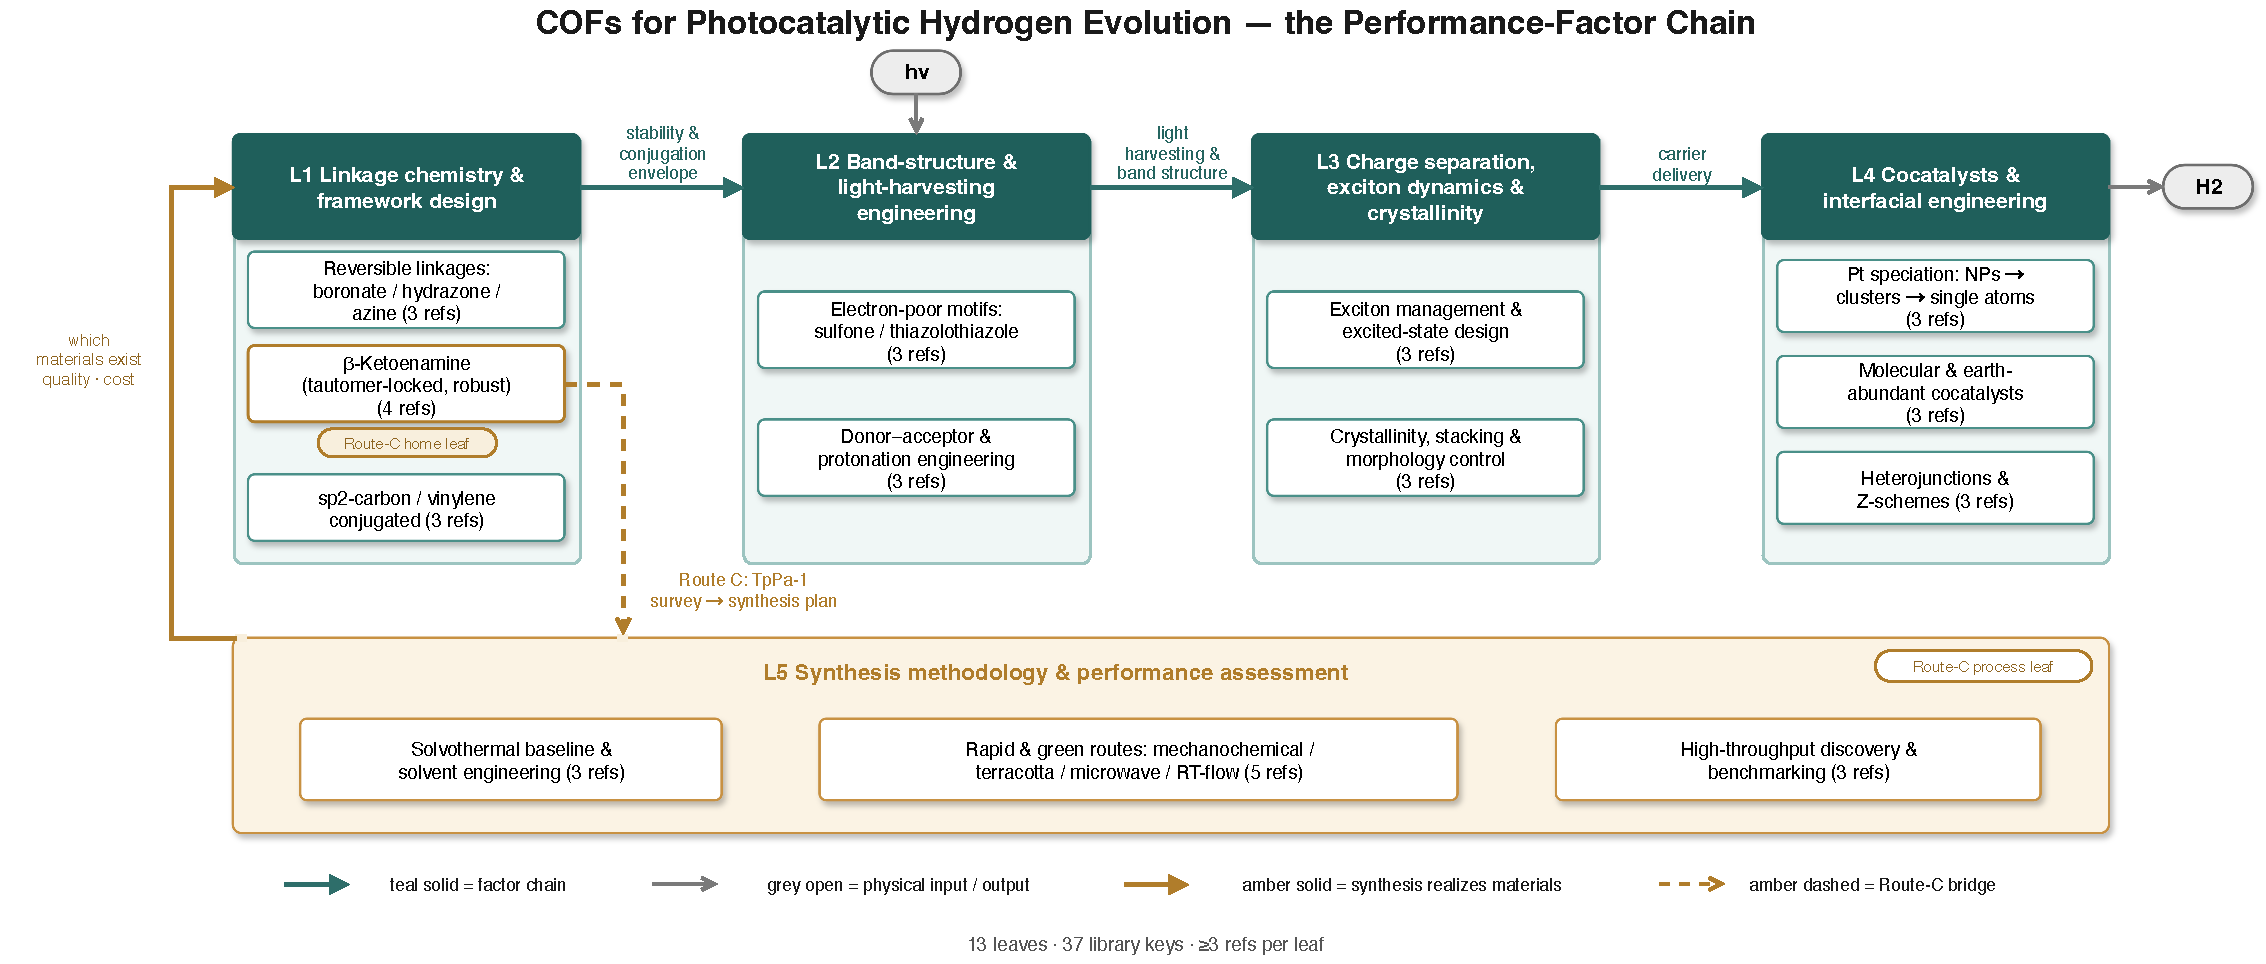
\includegraphics[width=\linewidth]{figures/fig1_factor_chain.pdf}
  \caption{Factor-chain taxonomy of COF photocatalysts for the hydrogen evolution reaction
  (HER). Top: five groups of design levers (L1--L5) identified in this survey; bottom: the
  photon-to-H$_2$ physical pipeline. Labeled arrows mark the pipeline stage each lever family
  principally governs; the synthesis level (L5) acts indirectly by setting crystallinity and
  phase purity.}
  \label{fig:factorchain}
\end{figure}

Scope follows the audited protocol of this project: crystalline 2D/3D COFs evaluated for
sacrificial photocatalytic HER, plus synthesis-methodology studies of the TpPa family required
by C3; metal--organic frameworks, CO$_2$ photoreduction, and pure oxygen-evolution studies are
excluded. All 37 cited references were retrieved by multi-source search (arXiv, OpenAlex,
Crossref) and passed a zero-tolerance citation-integrity audit; the audit trail is part of the
deliverable. The survey is written for materials and chemistry graduate students: the intended
takeaway is a mental model of \emph{which factor limits which performance regime}, plus a
reusable template for turning literature evidence into a synthesis decision.

\section{Design levers I: linkage chemistry and band-structure engineering}
\label{sec:levers}

\subsection{L1 --- Linkage chemistry sets the stability--crystallinity envelope}
\label{sec:linkage}

The linkage is the first and most consequential design decision, because it fixes both the
chemical stability envelope and the degree of $\pi$-conjugation available to every downstream
lever. COF linkage design is governed by a now well-articulated trade-off: reversible bond
formation enables the error correction that produces crystallinity, but the same reversibility
makes the framework hydrolytically fragile~\cite{haase2020solving}. The field's linkage history
is a sequence of answers to this trilemma.

\textbf{Reversible foundations (L1a).} Boronate-ester frameworks demonstrated that purely
organic building blocks can crystallize into predictable lattices~\cite{cote2005porous}, but
their boron--oxygen bonds hydrolyze readily, which confines them to anhydrous
applications~\cite{cote2005porous,haase2020solving}. Hydrazone linkages brought the first
photocatalytic milestone: TFPT-COF evolved hydrogen from water with a sacrificial donor and Pt
cocatalyst~\cite{stegbauer2014a}. Azine linkages then delivered an early systematic
structure--activity series: in the N$_x$-COF platform, HER activity rises monotonically with
the number of ring nitrogens (N3 $>$ N2 $>$ N1 $>$ N0), demonstrating that atomically
precise framework chemistry translates into tunable photocatalysis~\cite{vyas2015a}.

\textbf{$\beta$-Ketoenamine lock (L1b).} The TpPa family resolved the stability half of the
trilemma with a two-stage thermodynamic design: reversible Schiff-base condensation of
1,3,5-triformylphloroglucinol (Tp) with \emph{p}-phenylenediamine (Pa-1) in 1:1
mesitylene/dioxane first builds a crystalline enol-imine network, which then undergoes an
\emph{irreversible} enol$\rightarrow$keto tautomerization; only the keto form is observed, and
the resulting TpPa-1 survives 9~N HCl and boiling water~\cite{kandambeth2012construction}.
Because the lock is chemical rather than processual, it survives radically different syntheses:
room-temperature solvent-free grinding gives the same stable frameworks, albeit with moderate
crystallinity and an exfoliated, graphene-like morphology~\cite{biswal2013mechanochemical}.
The scaffold is also a productive photocatalysis platform: acetylene- and diacetylene-walled
$\beta$-ketoenamine COFs show that extending wall conjugation markedly raises HER (the
diacetylene analogue outperforms the acetylene one)~\cite{pachfule2017diacetylene}, and a
fixed-backbone substituent series (TpPa-COF-X, X = --H, --(CH$_3$)$_2$, --NO$_2$) maps how
peripheral electronics shift morphology, light absorption, and activity~\cite{sheng2019effect}.
This chemistry is the home leaf of the Route~C target (Sec.~\ref{sec:routec}).

\textbf{Fully conjugated linkages (L1c).} Vinylene (sp$^2$-carbon) linkages remove the
conjugation bottleneck of C--N single bonds. sp$^2$-carbon-conjugated frameworks have been
applied to photocatalytic hydrogen production~\cite{jin20192d}; mild Knoevenagel
polycondensation now affords vinylene-linked benzobisthiazole frameworks
(BTH-1/2/3)~\cite{wang2022facile}, and benzothiazole-mediated aldol-type polycondensation
yields unsubstituted-vinylene 2D COFs whose two-dimensional frameworks outperform their 1D
counterparts in photocatalysis~\cite{li2023two}. The cost is narrower monomer scope and
condition-sensitive synthesis~\cite{wang2022facile,li2023two}.

Read as a series, L1 shows the trilemma being solved twice over: the $\beta$-ketoenamine
route buys hydrolytic stability by spending linkage reversibility \emph{after} crystallization
has already happened~\cite{kandambeth2012construction}, whereas the vinylene route accepts a
harder crystallization problem up front in exchange for uninterrupted
conjugation~\cite{li2023two,haase2020solving}. Which trade is better is not decidable at the
linkage level alone --- it depends on whether the downstream bottleneck is carrier transport or
framework survival, which is precisely why this survey tracks the full factor chain rather
than ranking linkages in isolation~\cite{haase2020solving,zhang2022reconstructed}.

\begin{table}[t]
\centering
\caption{Linkage classes for COF HER photocatalysts (taxonomy level L1). Stability and
activity statements are those reported in the cited studies.}
\label{tab:linkage}
\footnotesize
\begin{tabular}{p{2.3cm}p{2.4cm}p{3.3cm}p{4.9cm}}
\toprule
Linkage class & Exemplar & Formation chemistry & Reported stability / HER relevance \\
\midrule
Boronate ester (L1a) & COF-1, COF-5~\cite{cote2005porous} & Boronic acid + catechol
condensation & Thermally robust; hydrolytically labile~\cite{cote2005porous,haase2020solving} \\
Hydrazone (L1a) & TFPT-COF~\cite{stegbauer2014a} & Aldehyde + hydrazide & First COF HER
demonstration~\cite{stegbauer2014a} \\
Azine (L1a) & N$_x$-COF~\cite{vyas2015a} & Aldehyde + hydrazine & Water/photo-stable; HER
scales with N count~\cite{vyas2015a} \\
$\beta$-Ketoenamine (L1b) & TpPa-1/-2~\cite{kandambeth2012construction} & Reversible imine +
irreversible tautomerization & 9~N HCl, boiling water (9~N NaOH for
TpPa-2)~\cite{kandambeth2012construction}; HER platform~\cite{pachfule2017diacetylene,sheng2019effect} \\
Vinylene / sp$^2$-C (L1c) & BTH-1/2/3~\cite{wang2022facile};
v-2D-COF-NS~\cite{li2023two} & Knoevenagel / aldol-type polycondensation & Full in-plane
conjugation; 2D $>$ 1D photocatalysis~\cite{li2023two} \\
\bottomrule
\end{tabular}
\end{table}

\subsection{L2 --- Band-structure and light-harvesting engineering}
\label{sec:band}

With the linkage fixed, the second lever tunes what the framework absorbs and how strongly
photogenerated excitons are pulled apart. Two motifs dominate the library evidence.

\textbf{Electron-poor heteroaromatics (L2a).} Sulfone chemistry produced one of the field's
benchmark materials: the dibenzothiophene-sulfone framework FS-COF for hydrogen evolution from
water~\cite{wang2018sulfone}. Its significance was consolidated by a factor-deconvolution study
on the same family, which varied band gap, crystallinity, surface area, exciton migration, and
charge extraction quasi-independently and identified crystallinity and charge extraction as the
prime factors --- a rare causal, rather than correlational, result in this
literature~\cite{ghosh2020identification}. Thiazolo[5,4-d]thiazole acceptors paired with pyrene
donors (PyTz-COF) show that a bicontinuous donor/acceptor channel architecture underlies the
exceptional optoelectronic response~\cite{li2020thiazolo}.

\textbf{Donor--acceptor construction and post-synthetic protonation (L2b).} Multicomponent
synthesis extends the D--A idea to three components: triazine acceptors and benzotrithiophene
donors bridged by sp$^2$-carbon links boost HER beyond two-component
controls~\cite{li2023three}. Post-synthetic linkage protonation of imine D--A COFs red-shifts
absorption and improves charge separation, reaching 20.7~mmol\,g$^{-1}$\,h$^{-1}$
~\cite{yang2021protonated}. In exfoliated form, a $\beta$-ketene--cyano D--A pair in COF
nanosheets couples dramatically prolonged carrier lifetimes (femtosecond transient absorption
evidence) with an AQE of 82.6\% at 450~nm --- currently the clearest demonstration that L2
engineering, executed on an L1-stable scaffold and read out through L3 photophysics, produces
step-change activity~\cite{li2022covalent}.

\section{Design levers II: charge management and interfacial catalysis}
\label{sec:charge}

\subsection{L3 --- Excitons, crystallinity, and stacking order}
\label{sec:excitons}

Absorbed photons in organic frameworks yield strongly bound excitons, so the third lever is
whether those excitons dissociate and whether the resulting charges survive transport.
Mechanistic perspectives now treat photon absorption, exciton dissociation, and electron
delivery as separately measurable stages of one pipeline~\cite{blatte2024photons}.

\textbf{Excited-state design (L3a).} Computation has moved upstream of synthesis:
density-functional screening across donor--acceptor pairs shows the exciton binding energy
$E_b$ is systematically tunable through D--A strength, making $E_b$ a design variable rather
than a post-hoc measurement~\cite{qian2023computation}. On the experimental side, an
isoreticular hydrazide-COF series resolved how excited-state electron distribution and
transport pathways change with the linker, tying photophysics to specific framework
positions~\cite{chen2023tuning}. What is still missing is the closed loop between the two
communities --- computed $E_b$ values validated by spectroscopy on the same material series
(Sec.~\ref{sec:challenges}, G5)~\cite{qian2023computation,chen2023tuning,blatte2024photons}.

\textbf{Crystallinity and stacking (L3b).} The factor-deconvolution benchmark identified
crystallinity as a prime HER factor~\cite{ghosh2020identification}, and two complementary
studies show why and how to act on it. During photocatalytic cycling, coaxial stacking can
disorder and activity decays; threading poly(ethylene glycol) through the mesopores locks the
stacked configuration and prevents the decline~\cite{zhou2021peg} --- direct evidence that
\emph{operando} structural integrity, not just as-made crystallinity, matters. At the synthesis
end, the reconstruction strategy decouples polymerization from crystallization: amorphous
imine networks pre-organized by a removable covalent tether reconstruct into highly crystalline
frameworks, lifting sacrificial HER to 27.98~mmol\,h$^{-1}$\,g$^{-1}$ --- the highest
sacrificial rate in this survey's library --- while confirming that poor reversibility of
robust linkages is the central obstacle the field must engineer
around~\cite{zhang2022reconstructed,haase2020solving}.

\subsection{L4 --- Cocatalysts and interfacial engineering}
\label{sec:interface}

Even perfectly delivered electrons produce no hydrogen without an interface that turns them
over. The library evidence organizes into three interface strategies.

\textbf{Pt speciation (L4a).} Platinum remains the default electron sink, but its speciation is
now a lever in its own right: dispersing Pt as single atoms on a COF raises active-site density
relative to nanoparticles~\cite{dong2021platinum}, while in-situ photodeposition yields
cluster-scale Pt with strong electronic coupling to the framework~\cite{li2022in}. The
factor-deconvolution protocol treats Pt loading and speciation as one of the deconvoluted
variables, which is what makes cross-material activity comparisons meaningful at
all~\cite{ghosh2020identification}.

\textbf{Molecular and earth-abundant cocatalysts (L4b).} The azine N$_2$-COF paired with a
chloro(pyridine)cobaloxime delivers 782~$\mu$mol\,h$^{-1}$\,g$^{-1}$ at a turnover number of
54.4, with mechanistic analysis supporting outer-sphere electron transfer to a monometallic
cobalt pathway~\cite{banerjee2017single}. Covalently wiring the cobaloxime to the backbone
improves and prolongs activity relative to physisorbed analogues by enabling recoordination of
the cocatalyst during operation~\cite{gottschling2020rational}. These molecular systems remain
orders of magnitude below Pt-based benchmarks in rate and turnover
(cf.~\cite{yang2021protonated}), a gap analyzed in Sec.~\ref{sec:challenges}
(G6)~\cite{banerjee2017single,gottschling2020rational}. Interface design more broadly ---
including cocatalyst anchoring chemistry --- is a central theme of the 2024 Accounts
survey~\cite{chen2024photocatalysis}.

\textbf{The sacrificial-system context.} Almost all quantitative claims in this section are
measured against sacrificial electron donors, and the donor is itself an interface-level
variable: the cobaloxime/N$_2$-COF benchmark operates with triethanolamine in a
water/acetonitrile medium~\cite{banerjee2017single}, while the record-setting protonated D--A
systems were developed in ascorbic-acid media, where the donor also participates in the
protonation equilibrium that red-shifts absorption~\cite{yang2021protonated}. Cross-study
comparisons that ignore the donor identity therefore conflate interfacial kinetics with donor
thermodynamics --- one of the reasons a fixed-protocol benchmark is registered as gap G1 in
Sec.~\ref{sec:challenges}~\cite{ghosh2020identification,banerjee2017single}.

\textbf{Heterojunctions and Z-schemes (L4c).} Coupling COFs to inorganic partners re-routes
charges across a built-in junction: an in-situ grown, chemically bonded 2D/2D COF /
oxygen-vacancy-WO$_3$ Z-scheme targets \emph{overall} water splitting rather than sacrificial
HER~\cite{shen2023in}, and a 2D/2D COF/CdS Z-scheme heterojunction enhances photocatalytic
hydrogen evolution~\cite{gao20222d}. Composite and heterojunction photocatalysts are surveyed
systematically in the 2020 CSR review~\cite{wang2020covalent}. The overall-water-splitting
rates remain far below sacrificial benchmarks~\cite{shen2023in}, marking the sacrificial-donor
dependency as a field-level open problem (Sec.~\ref{sec:challenges}, G2).

Taken together, L3 and L4 close the causal chain begun in Sec.~\ref{sec:levers}: linkage and
band engineering determine what can be absorbed and separated; crystallinity, stacking, and the
catalytic interface determine how much of that potential is converted. The prime-factor
evidence~\cite{ghosh2020identification} justifies the ordering used in the synthesis design of
Sec.~\ref{sec:routec}: crystallinity first, interface second, everything else after.

\section{Synthesis methodology: five routes to the same framework}
\label{sec:synthesis}

The final lever (L5) is often treated as logistics, but the library evidence says otherwise:
the synthesis route sets the crystallinity and phase purity on which every upstream factor
depends~\cite{ghosh2020identification,zhang2022reconstructed}. This section compares the five
route families documented for the TpPa system, the target chemistry of Route~C.

\textbf{Solvothermal baseline and solvent thermodynamics (L5a).} The canonical TpPa-1 protocol
--- Tp + Pa-1 in 1:1 mesitylene/dioxane with aqueous acetic acid, sealed at 120~$^\circ$C for
72~h --- remains the reference for crystallinity and chemical
robustness~\cite{kandambeth2012construction}. Solvent choice, long empirical, now has a
quantitative decision framework: ranking solvents by CHEM21 greenness, Hansen solubility
parameters, and free energy of solvation shows that moderate-solvation media (1,4-dioxane,
propylene carbonate, diacetin) suppress excessive reaction reversibility and promote
crystallite growth~\cite{xu2026structural}. New synthetic strategies across the COF field are
compiled in the dedicated CSR review~\cite{li2020new}.

\textbf{Rapid and green routes (L5b).} Four alternatives trade conditions against quality:
\begin{itemize}
\item \emph{Mechanochemical grinding}: room-temperature, solvent-free, delivering the same
  chemical stability with moderate crystallinity and partially exfoliated
  morphology~\cite{biswal2013mechanochemical}.
\item \emph{Salt-mediated (``organic terracotta'')}: p-toluenesulfonic acid mediation
  crystallizes ultraporous frameworks in seconds, with family surface areas up to
  3000~m$^2$\,g$^{-1}$ and continuous processing demonstrated on a twin-screw
  extruder~\cite{karak2017constructing}.
\item \emph{Microwave-assisted solvothermal}: an enamine COF forms in significantly less time
  at lower temperature with high yield~\cite{wei2015the}; in the direct TpPa-1 comparison
  compiled by the microwave review, 1~h at 100~$^\circ$C gives a BET surface area of
  725~m$^2$\,g$^{-1}$ versus 152~m$^2$\,g$^{-1}$ for the conventional 3-day, 120~$^\circ$C
  control~\cite{grenu2020microwave}. The same review documents an instructive caveat: for
  transimination-based crystallinity upgrading, solvothermal heating still outperforms
  microwave for $\beta$-ketoenamine COFs --- the ``fastest route'' is
  context-dependent~\cite{grenu2020microwave}.
\item \emph{Room-temperature and flow synthesis}: RT batch TpPa-1 matches solvothermal
  crystallinity and porosity, attributed to monomer solubility and $\pi$-stacking-assisted
  error correction; the first continuous-flow COF production reached 41~mg\,h$^{-1}$ at a
  space-time yield of 703~kg\,m$^{-3}$\,day$^{-1}$~\cite{peng2016room}. Flow synthesis of
  TpPa-1 in the green solvent diacetin reaches a BET area of 418~m$^2$\,g$^{-1}$ with a
  30-fold space-time-yield increase and an 89\% reduction in specific energy relative to batch
  in the same solvent~\cite{xu2026structural}.
\end{itemize}

\textbf{High-throughput discovery (L5c).} Scale-out of synthesis itself is emerging:
sonochemical high-throughput experimentation screened 76 polymers, of which 60 formed
crystalline COFs and 18 were previously unreported, in a single campaign --- the target
application was photocatalytic H$_2$O$_2$ production, but the accelerated
synthesis-plus-screening methodology transfers directly to HER~\cite{zhao2022accelerated}.
The campaign format matters for this survey's argument: it is the first library-scale
demonstration that route parameters (here, sonication) can be co-screened with photocatalytic
output, rather than fixed by convention before testing begins~\cite{zhao2022accelerated}.
Combined with AQE-standardized reporting~\cite{li2022covalent} and factor
benchmarking~\cite{ghosh2020identification}, this points toward synthesis--performance maps
built at campaign scale rather than paper scale.

\begin{table}[t]
\centering
\caption{Synthesis routes to TpPa-family COFs (taxonomy level L5). Quantities are as reported
in the cited sources; dashes mark values not reported in the library evidence.}
\label{tab:routes}
\footnotesize
\begin{tabular}{p{2.7cm}p{3.1cm}p{3.5cm}p{3.6cm}}
\toprule
Route & Conditions & Reported quality & Scale/greenness notes \\
\midrule
Solvothermal~\cite{kandambeth2012construction} & 120~$^\circ$C, 72~h,
mesitylene/dioxane + aq.~AcOH & Reference crystallinity; 9~N HCl and boiling-water stability &
Sealed-tube batch; high-boiling solvents \\
Mechanochemical~\cite{biswal2013mechanochemical} & Room temperature, solvent-free grinding &
Moderate crystallinity; stability retained; exfoliated layers & Greenest inputs; lowest
crystallinity \\
Salt-mediated~\cite{karak2017constructing} & p-TsOH mediation, seconds & Highly crystalline,
ultraporous (up to 3000~m$^2$\,g$^{-1}$, family value) & Twin-screw extrusion; salt work-up
required \\
Microwave~\cite{wei2015the,grenu2020microwave} & 100~$^\circ$C, 1~h & BET 725 vs.\
152~m$^2$\,g$^{-1}$ (conventional control) & Fastest lab route; penetration-depth scale limit \\
RT / flow~\cite{peng2016room,xu2026structural} & RT batch; flow in diacetin & RT: comparable to
solvothermal; flow: BET 418~m$^2$\,g$^{-1}$ & Flow: 30$\times$ STY, $-$89\% specific energy;
COF flow precedent 703~kg\,m$^{-3}$\,day$^{-1}$ \\
\bottomrule
\end{tabular}
\end{table}

The pattern across Table~\ref{tab:routes} motivates the design task of the next section: no
single route dominates all axes, and the HER consequences of the green/scalable routes are
essentially unmeasured (Sec.~\ref{sec:challenges}, G4). Choosing a route is therefore a
decision problem with documented trade-offs --- exactly the kind of problem a survey should
hand over to synthesis planning in executable form.

\section{Synthesis design (Route C): from factor chain to a TpPa-1 protocol}
\label{sec:routec}

This section converts the survey's evidence into a decision-recorded synthesis plan for the
$\beta$-ketoenamine COF TpPa-1 (monomers: 1,3,5-triformylphloroglucinol, Tp; and
\emph{p}-phenylenediamine, Pa-1; stoichiometry 2\,Tp\,:\,3\,Pa-1 from the 3$\times$CHO /
2$\times$NH$_2$ functional balance)~\cite{kandambeth2012construction}. The full
safety-annotated protocol, candidate-route decision table, and machine-readable experiment plan
are deliverable artifacts of this project;\footnote{Artifacts:
\texttt{ideas/route\_c\_synthesis\_plan.md} and \texttt{ideas/experiment\_route\_c\_tppa1.json}
in the project workspace.} this section presents the decision logic and the quantitative core. Figure~\ref{fig:route} shows the route.

\begin{figure}[t]
  \centering
  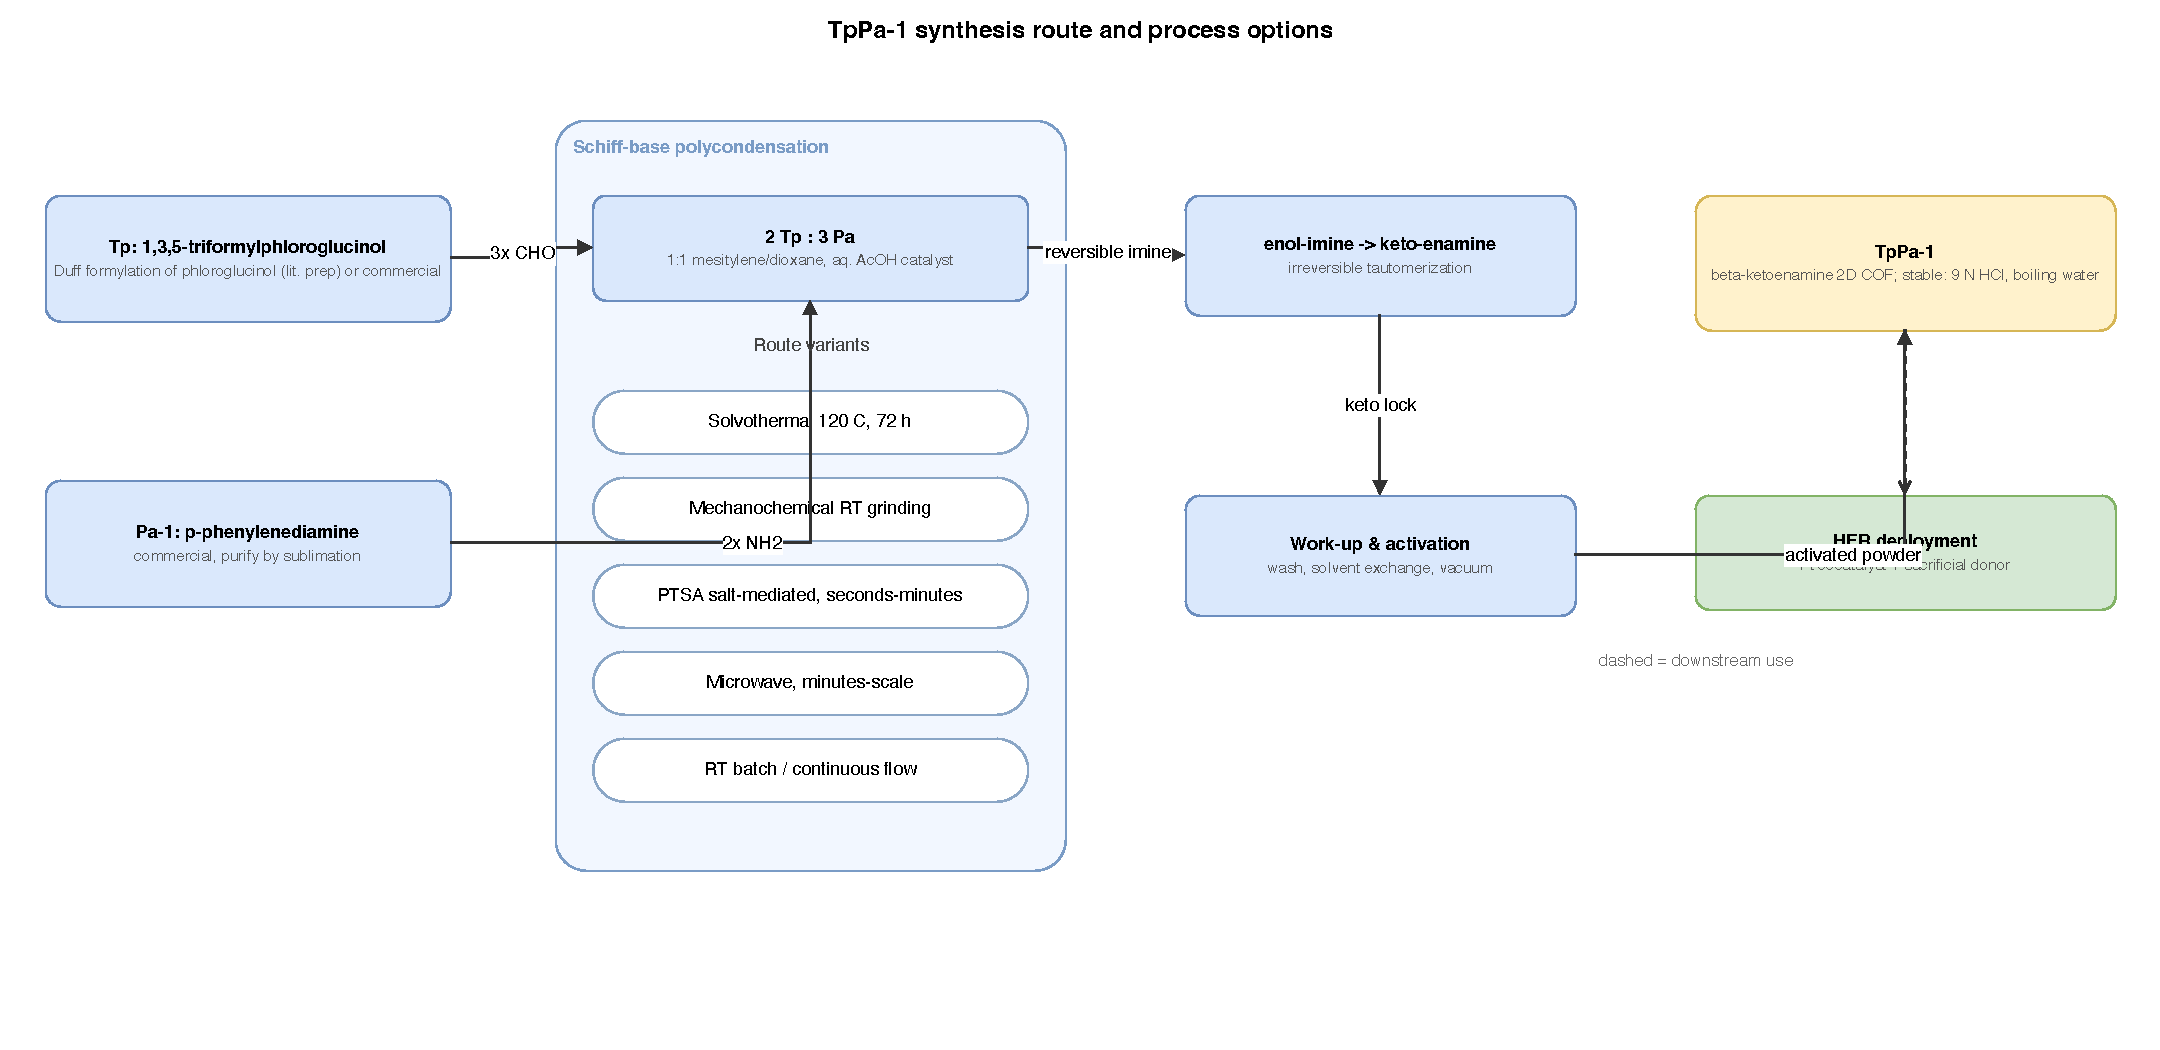
\includegraphics[width=\linewidth]{figures/fig2_tppa1_route.pdf}
  \caption{Synthesis of TpPa-1. Monomers condense via reversible Schiff-base chemistry (route
  variants shown as chips; quantitative comparison in Table~\ref{tab:routes}) and lock into the
  $\beta$-ketoenamine form by irreversible tautomerization, giving an
  acid/base/boiling-water-stable framework deployable for photocatalytic HER.}
  \label{fig:route}
\end{figure}

\textbf{Why TpPa-1, and why these criteria.} The factor chain orders the design requirements:
crystallinity and charge extraction are the prime activity factors~\cite{ghosh2020identification},
and aqueous photocatalysis presupposes hydrolytic stability, which the irreversible
enol$\rightarrow$keto lock provides at the linkage level~\cite{kandambeth2012construction,haase2020solving}.
TpPa-1 is also the only COF in the library with five independently documented synthesis routes
(Table~\ref{tab:routes}), making it the strongest available testbed for evidence-based process
selection~\cite{kandambeth2012construction,biswal2013mechanochemical,karak2017constructing,wei2015the,peng2016room,xu2026structural}.

\textbf{Baseline protocol (decision: solvothermal R1).} Monomer quality first: Pa-1 is
purified (sublimation) immediately before use --- a chemical-practice inference consistent with
the observation that monomer solubility and purity enable mild-condition
growth~\cite{peng2016room}; Tp is purchased or prepared by the literature Duff-type formylation
of phloroglucinol~\cite{kandambeth2012construction}. Condensation follows the origin protocol
(1:1 mesitylene/dioxane, aqueous AcOH, 120~$^\circ$C, 72~h, sealed
tube)~\cite{kandambeth2012construction}, chosen over the four alternatives because it carries
the richest characterization record against which optimized batches can be compared
(Table~\ref{tab:routes}). Work-up uses solvent washing, solvent exchange, and vacuum
activation~\cite{kandambeth2012construction,karak2017constructing}. Deployment for HER follows
the TpPa-COF-X benchmark configuration (in-situ Pt photodeposition, sacrificial
donor)~\cite{sheng2019effect}, with Pt speciation tunable as an independent
factor~\cite{dong2021platinum,li2022in}.

\textbf{Optimization O1 --- microwave heating.} Replacing oven heating with microwave
irradiation reduces reaction time from 72~h to 1~h and temperature from 120 to 100~$^\circ$C
while \emph{increasing} the BET surface area from 152 to 725~m$^2$\,g$^{-1}$ in the direct
comparison~\cite{wei2015the,grenu2020microwave} --- a 98.6\% time reduction and a
$\sim$4.8$\times$ porosity gain. The documented caveat (solvothermal beats microwave for
transimination-based upgrading of $\beta$-ketoenamine COFs~\cite{grenu2020microwave}) is
recorded in the decision table: O1 optimizes the \emph{direct} route, not every quality
pathway.

\textbf{Optimization O2 --- green-solvent continuous flow.} The solvent-thermodynamics
framework (CHEM21 greenness, Hansen parameters, free energy of solvation) selects diacetin;
flow-derived TpPa-1 reaches a BET area of 418~m$^2$\,g$^{-1}$, a 30-fold space-time-yield
increase, and an 89\% reduction in specific energy versus batch in the same
solvent~\cite{xu2026structural}. Feasibility rests on the demonstrated room-temperature growth
of TpPa-1 with solvothermal-grade quality and on the flow precedent of
703~kg\,m$^{-3}$\,day$^{-1}$~\cite{peng2016room}. A salt-mediated seconds-scale route is held
in reserve for crystallinity rescue at scale~\cite{karak2017constructing}, with
amorphous-to-crystalline reconstruction as a further fallback
paradigm~\cite{zhang2022reconstructed}.

\textbf{Thermodynamic feasibility audit.} Literature-supported statements: (i) the route is a
reversible imine equilibrium (error-correcting, crystallinity-enabling) feeding an irreversible
tautomerization whose keto product is the only observed form --- a thermodynamic
sink~\cite{kandambeth2012construction}; (ii) retained crystallinity in 9~N HCl and boiling
water evidences the depth of that sink~\cite{kandambeth2012construction,biswal2013mechanochemical};
(iii) moderate-solvation media thermodynamically balance reversibility against crystallite
growth~\cite{xu2026structural}; (iv) the general reversibility--crystallinity--stability
trade-off frames why this two-stage design is necessary at
all~\cite{haase2020solving,zhang2022reconstructed}. Quantities \emph{not} reported in the
library --- keto/enol tautomer energetics, per-bond condensation free energy, periodic
formation and stacking energies, monomer solvation free energies --- are deliberately left as a
to-be-computed list with recommended DFT setups (dispersion-corrected hybrid functionals with
implicit solvation for molecular models; dispersion-corrected periodic PBE for the framework;
COSMO-RS for solvation screening) rather than asserted numerically. No numeric value in this
section originates outside the cited sources.

\textbf{Validation and characterization plan.} Every batch is judged against
literature-anchored acceptance criteria: powder X-ray diffraction against the simulated
pattern establishes crystallinity~\cite{kandambeth2012construction}; FT-IR and $^{13}$C
CP-MAS NMR must show the keto-form signature that certifies complete
tautomerization~\cite{kandambeth2012construction}; nitrogen sorption benchmarks porosity
against the 725~m$^2$\,g$^{-1}$ (microwave) and 418~m$^2$\,g$^{-1}$ (flow) reference
values~\cite{grenu2020microwave,xu2026structural}; and a 9~N HCl / boiling-water soak with
post-treatment diffraction reproduces the origin stability test~\cite{kandambeth2012construction}.
Stacking disorder during photocatalytic cycling is monitored as a separate failure mode,
following the operando evidence~\cite{zhou2021peg}. Because the three production routes (R1,
O1, O2) will be characterized under one protocol and then deployed under the same HER
configuration~\cite{sheng2019effect}, the plan doubles as the seed experiment for gap G4 ---
the missing route$\rightarrow$crystallinity$\rightarrow$HER chain
(Sec.~\ref{sec:challenges})~\cite{ghosh2020identification}.

\textbf{Safety and integration notes.} The deliverable protocol carries a mandatory hazard
table (diamine sensitizer, dioxane peroxide former, sealed-vessel pressure, microwave-rated
reactors only~\cite{grenu2020microwave}, H$_2$/O$_2$ explosion limits during photocatalysis,
acid handling for in-house Tp preparation). A retrosynthesis-backend integration demo (stub
provider) is included in the project state \emph{explicitly labeled as demonstration data, not
chemical conclusions}; all chemistry above traces to the audited literature.

\section{Open challenges: an evidence-chained gap register}
\label{sec:challenges}

Each gap below is grounded in at least two audited references, annotated with the database that
surfaced the evidence (arXiv / OpenAlex / Crossref, per the project search log), and closed
with the reasoning why current work leaves it open. The register is maintained as a standalone
deliverable (\texttt{notes/research\_gaps.md}) and summarized here.

\textbf{G1 --- No standardized cross-family HER benchmark.} Factor deconvolution exists within
a single family (S-COF/FS-COF; OpenAlex)~\cite{ghosh2020identification}, while performance is
reported in incommensurable currencies --- AQE at a stated wavelength
(OpenAlex)~\cite{li2022covalent} versus mass-normalized rates
(OpenAlex)~\cite{yang2021protonated} --- and high-throughput screening has targeted H$_2$O$_2$
rather than HER (OpenAlex)~\cite{zhao2022accelerated}. \emph{Why open:} multi-variable control
samples are costly, and reporting conventions differ across groups --- the same library
contains AQE-denominated and mass-rate-denominated headline results with no conversion
basis~\cite{li2022covalent,yang2021protonated}; no library study runs two linkage families
under one fixed protocol. \emph{Needed:} a fixed-protocol,
multi-family benchmark reporting both AQE and mass rate.

\textbf{G2 --- Overall water splitting remains a single-example regime.} The only library
system targeting non-sacrificial operation is the chemically bonded 2D/2D COF/WO$_3$ Z-scheme,
with rates far below sacrificial benchmarks (OpenAlex)~\cite{shen2023in}; the 2020 CSR review
confirms sacrificial dominance across COF photocatalysis (OpenAlex/Crossref)~\cite{wang2020covalent};
even molecular-cocatalyst systems rely on sacrificial donors (OpenAlex)~\cite{banerjee2017single}.
\emph{Why open:} sacrificial donors mask the four-electron oxidation half-reaction, whose
oxidative stress and band-position demands most COFs were never designed to meet.
\emph{Needed:} valence-band and anti-oxidation engineering plus Z-scheme charge routing
designed for the OER half-reaction.

\textbf{G3 --- Operando structural durability is unquantified.} Coaxial stacking disorders
during photocatalytic cycling and activity decays unless the stack is locked
(OpenAlex)~\cite{zhou2021peg}; chemical stability tests (9~N HCl, boiling water;
Crossref)~\cite{kandambeth2012construction} probe a different failure axis, and the
linkage-design trilemma contains no operando dimension (OpenAlex)~\cite{haase2020solving}.
\emph{Why open:} the field equates chemical with photocatalytic stability, and standard
practice is before/after PXRD rather than time-resolved structural tracking. \emph{Needed:}
operando structure--activity correlation (cycles vs.\ crystallinity vs.\ rate) and a shared
``photocatalytic lifetime'' reporting convention.

\textbf{G4 --- Green and scalable routes are not HER-benchmarked.} Flow-derived TpPa-1 reports
BET area, space-time yield, and energy metrics but no HER data
(Crossref)~\cite{xu2026structural}; the microwave comparison stops at porosity and CO$_2$
uptake (OpenAlex)~\cite{grenu2020microwave,wei2015the}; room-temperature and flow routes close
with crystallinity and porosity (OpenAlex)~\cite{peng2016room}. \emph{Why open:} the synthesis
methodology and photocatalysis communities publish to different completion criteria, so the
route$\rightarrow$crystallinity$\rightarrow$HER chain --- whose middle link is causally
established (OpenAlex)~\cite{ghosh2020identification} --- has never been closed on one
material. \emph{Needed:} same-protocol HER comparison of solvothermal, microwave, flow, and
mechanochemical TpPa-1 --- precisely the experiment Route~C (Sec.~\ref{sec:routec}) is designed
to seed.

\textbf{G5 --- Exciton-binding-energy design rules lack an experimental loop.} DFT screening
makes $E_b$ tunable on paper (OpenAlex)~\cite{qian2023computation}; excited-state mapping is
family-specific (OpenAlex)~\cite{chen2023tuning}; and the mechanistic perspective explicitly
calls the pipeline's characterization methodology unsettled (OpenAlex)~\cite{blatte2024photons}.
\emph{Why open:} measuring $E_b$ on polycrystalline powders is noisy and mismatched to idealized
computational models, and computational and spectroscopic groups rarely share sample sets.
\emph{Needed:} a computed-then-measured $E_b$ benchmark across one isoreticular series.

\textbf{G6 --- Earth-abundant cocatalysts trail Pt by orders of magnitude.} The
cobaloxime/N$_2$-COF system achieves 782~$\mu$mol\,h$^{-1}$\,g$^{-1}$ at TON 54.4
(OpenAlex)~\cite{banerjee2017single}; covalent wiring prolongs but does not eliminate
degradation (OpenAlex)~\cite{gottschling2020rational}; meanwhile the field's effort
concentrates on Pt speciation (OpenAlex)~\cite{dong2021platinum,li2022in}. \emph{Why open:}
molecular-cocatalyst failure modes demand operando spectro-electrochemistry beyond most COF
groups' stacks, while Pt photodeposition is operationally trivial. \emph{Needed:} self-healing
ligand design on covalent anchors, and lifecycle TON accounting that makes the Pt/non-Pt
comparison honest.

These six gaps are not independent: G1's protocol deficit blocks progress measurement on G2--G6,
and G4 is the gap this survey's Route~C plan directly operationalizes. The gap register with
full evidence chains and database provenance accompanies this survey as an audited deliverable.

\section{Conclusion}
\label{sec:conclusion}

This survey organized COF photocatalytic hydrogen evolution by performance factor rather than
material family. The factor chain --- linkage chemistry (L1), band engineering (L2), exciton
and order management (L3), interfacial catalysis (L4), synthesis methodology (L5) --- maps each
design lever to the pipeline stage it governs, with crystallinity and charge extraction
established as the prime factors by the field's clearest causal
benchmark~\cite{ghosh2020identification}. Along that chain, the $\beta$-ketoenamine tautomer
lock stands out as the load-bearing chemical innovation for aqueous operation: a reversible,
error-correcting condensation that ends in an irreversible, hydrolysis-proof
sink~\cite{kandambeth2012construction}.

The survey's second half converted that evidence into practice. The six-entry gap register
shows where the literature stops --- most actionably, the green and scalable synthesis routes
whose HER consequences remain unmeasured --- and the Route~C plan turns that specific gap into
an executable protocol: a solvothermal baseline with two quantified optimizations (microwave:
1~h at 100~$^\circ$C with a $\sim$4.8$\times$ porosity gain; green-solvent flow: 30$\times$
space-time yield at $-$89\% specific energy), a thermodynamic audit that refuses to invent
numbers, and a mandatory safety annex~\cite{grenu2020microwave,xu2026structural}.

The reader we designed for should leave with two assets: a mental model of which factor limits
which performance regime, and a worked template for converting survey evidence into a synthesis
decision --- the survey-to-synthesis bridge that the COF hydrogen-evolution field, now rich in
materials and mechanisms but poor in standardized decisions, most needs.


% paper-orchestra rule: flush all pending floats before the bibliography
\clearpage

\bibliographystyle{plainnat}
\bibliography{references}
\end{document}
